Tenemos la siguiente pila:
\begin{center}
    \begin{tabular}{|c|c|c|}
        \hline
        Estado actual & Siguientes estados y $h$ correspondientes & Cerrados\\
        \hline
        $s_0$ & $(s_2:3)$ & $s_0$ \\
        \hline
        $s_2$ & $(s_4:1), (s_1:2)$ & $s_0,s_2$ \\
        \hline
        $s_4$ & $(s_1:2), (s_3:2), (s_5:2)$ & $s_0,s_2,s_4$ \\
        \hline
        $s_1$ & $(s_3:2), (s_5:2)$ & $s_0,s_2,s_4,s_1$ \\
        \hline
        $s_3$ & $(s_5:2)$ & $s_0,s_2,s_4,s_1,s_3$ \\
        \hline
        $s_5$ & $(s_6:0) (s_7:0)$ & $s_0,s_2,s_4,s_1,s_3,s_5$ \\
        \hline
        $s_6$ & $(s_7:0)$ & $s_0,s_2,s_4,s_1,s_3,s_5,s_6$ \\
        \hline
        $s_7$ & Estado final & $s_0,s_2,s_4,s_1,s_3,s_5,s_6,s_7$ \\
        \hline
    \end{tabular}
\end{center}
Se tiene el siguiente árbol:
\begin{center}
    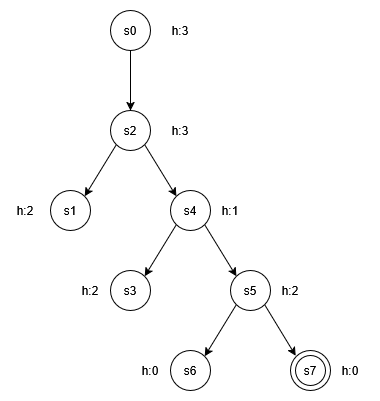
\includegraphics[height = 10cm]{respuestas/img/treeE7c.png}
\end{center}
Por lo que el camino solución es $a,b,b,a,a$, conformado por los estados $s_0,s_2,s_4,s_5,s_6,s_7$.